% Created 2020-03-05 Thu 19:37
% Intended LaTeX compiler: pdflatex
\documentclass[11pt]{article}
\usepackage[utf8]{inputenc}
\usepackage[T1]{fontenc}
\usepackage{graphicx}
\usepackage{grffile}
\usepackage{longtable}
\usepackage{wrapfig}
\usepackage{rotating}
\usepackage[normalem]{ulem}
\usepackage{amsmath}
\usepackage{textcomp}
\usepackage{amssymb}
\usepackage{capt-of}
\usepackage{hyperref}
\usepackage{tikz}
\usepackage[portuguese]{babel}
\usepackage[margin=1in]{geometry}
\usepackage{subcaption}
\author{Nícolas André da Costa Morazotti}
\date{\today}
\title{Lista Suplementar 1}
\hypersetup{
 pdfauthor={Nícolas André da Costa Morazotti},
 pdftitle={Lista Suplementar 1},
 pdfkeywords={},
 pdfsubject={},
 pdfcreator={Emacs 26.3 (Org mode 9.1.9)}, 
 pdflang={Portuguese}}
\begin{document}

\maketitle
\section{Questão 1}
\label{sec:org3781183}
É dado um sistema cartesiano \(\hat x\), \(\hat y\), \(\hat z\). Um fio reto
infinito, de raio \(a\) muito pequeno, se estende de \(z=-\infty\) a
\(z=\infty\). Calcule o campo elétrico num ponto P a uma distância \(r>a\) do
fio. \emph{Sugestão. Considere uma superfície imaginária cilíndrica cujo}
\emph{eixo coincide com o eixo \(z\), com raio \(r\) e comprimento \(L\) qualquer,}
\emph{de forma que o ponto \(P\) esteja na superfície cilíndrica. Argumente que o}
\emph{campo elétrico em \(P\) tem de ser perpendicular ao eixo z e}
\emph{radial. Aplique em seguida a Lei de Gauss à superfície cilíndrica.}

\begin{figure}[h!]
  \centering
  \begin{tikzpicture}
    \draw (0,0,0) circle (.2);
    \draw[dashed] (0,0,0) circle (1);
    \draw (-0.1,.17,0) -- (-0.1,.17,-4);
    \draw[dashed] (-0.6,0.8,0) -- (-0.5,0.9,-4);
    \draw (0.1,-.17,0) -- (0.1,-.17,-4);
    \draw[dashed] (0.8,-0.6,0) -- (0.9,-0.5,-4);
    \draw (0,0,-4) circle (.2);
    \draw[dashed] (0,0,-4) circle (1);
    \draw[->] (0,0,0) -- (0,0,3) node[left] {$z$};
    \filldraw[black] (-0.4,1,-1) circle (2pt) node[left] {$P$}
  \end{tikzpicture}
  \caption{Diagrama do exercício 1.}
  \label{fig:ex-1}
\end{figure}

Então, seja uma superfície gaussiana cilíndrica de raio \(r>a\), de
comprimento L. Podemos aplicar a Lei de Gauss
\begin{align*}
  \int \mathbf{E}\cdot d\mathbf{S} = \frac{Q_{in}}{\varepsilon_0}.
\end{align*}
Veja que, para um fio reto infinito carregado uniformemente com
densidade de carga \(\lambda\), cada ponto \((x,y,z)\) tem um ponto oposto
\((x,y,-z)\) com mesma carga. Assim, na componente \(z\), não pode haver
campo elétrico. Portanto, o campo elétrico deve ter apenas componentes
das direções \(\hat x\) e \(\hat y\).

Com um pouco mais de análise, vemos que o campo na verdade é na direção
\emph{radial} \(\hat\rho\). Assim,
\begin{align}
  \label{eq:1}
  \oint\mathbf E\cdot d\mathbf S &= |\mathbf E| 2\pi rL = \frac{Q_{in}}{\varepsilon_0}\\
                         &= \frac 1{\varepsilon_0}\int_{fio} dV \lambda\\
                         &= \frac {\lambda}{\varepsilon_0}\int_{fio} dV\\
                         &= \frac{\lambda\pi a^2L}{\varepsilon_0}\\
  |\mathbf E| &= \frac{\lambda a^2}{2\varepsilon_0 r}\\
  \mathbf E &= \hat\rho\frac{\lambda a^2}{2\varepsilon_0 r}.
\end{align}

\section{Questão 2}
\label{sec:org35731ff}
Num metal (condutor), o campo elétrico no interior do material é
necessariamente nulo; caso contrário, campo movimentaria eternamente as
cargas do metal. Mostre que as cargas elétricas num objeto metálico
somente podem estar na superfície do objeto. \emph{Sugestão. Dado um ponto}
\emph{\(P\) no interior do objeto, considere uma pequena superfície esférica,}
\emph{imaginária, centrada em \(P\). Aplique a Lei de Gauss a essa}
\emph{superfície.}

\begin{figure}[h!]
  \centering
  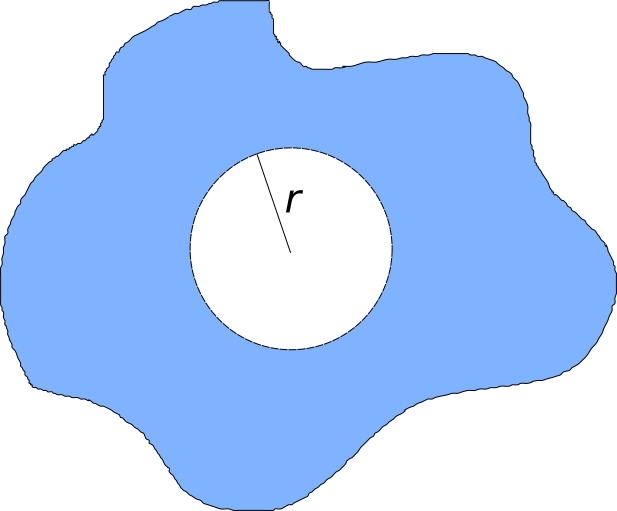
\includegraphics[scale=0.3]{imagens/ex-2.png}
  \caption{Em azul, um condutor sólido qualquer. Em branco, a
    superfície gaussiana de raio $r$ interna ao condutor. }
  \label{fig:ex-2}
\end{figure}

Considerando uma superfície gaussiana esférica de raio \(r\) interna ao
condutor, como visto na Figura \ref{fig:ex-2}, podemos ver que 
\begin{align*}
  \oint \mathbf E\cdot d\mathbf S &= \frac{Q_{in}}{\varepsilon_0}.
\end{align*}
Por construção, $\mathbf E \equiv 0$ dentro do condutor. Assim, a integral
é identicamente nula. 
\begin{align*}
  0 &\equiv \frac{Q_{in}}{\varepsilon_0}\\
  \implies Q_{in} &\equiv 0.
\end{align*}
Contudo, caso tenhamos uma superfície gaussiana externa ao condutor,
fica claro que o campo não é necessariamente \(0\), e portanto as cargas
devem se manter na superfície do condutor. 
\section{Questão 3}
\label{sec:org95a475c}
Uma placa metálica plana tem espessura uniforme \(2a\) e é infinita nas
outras direções. Posiciona-se um sistema cartesiano com os eixos \(x\) e
\(y\) paralelos à superfície da placa, de forma que a origem esteja no
plano central da placa. Assim, uma das superfícies da placa está no
plano \(z=a\), e a outra, no plano \(z = -a\). Sabe-se que as duas faces da
placa estão carregadas com densidade superficial \(\sigma\). Calcule o campo
elétrico num ponto sobre o eixo \(z\) na posição \((0,0,z_0)\), com \(z_0
>a\). Para isso, considere uma superfície imaginária cilíndrica cujo eixo
coincide com o eixo \(z\) e que tem tampas (paralelas ao plano \(xy\)) em
\(z=0\) (dentro do metal) e \(z=z_0\). Aplique a lei de Gauss a essa
superfície. 

\begin{figure}[h!]
  \begin{subfigure}{0.3\textwidth}
    \centering
    \begin{tikzpicture}
      \draw (0,-0.25,0) -- (0,-0.25,2.5) -- (2.5,-0.25,2.5) -- (2.5,-0.25,0) -- (0,-0.25,0);
      \draw[fill=white,opacity=0.8] (0,0.25,0) -- (0,0.25,2.5) -- (2.5,0.25,2.5) -- (2.5,0.25,0) -- (0,0.25,0);
      \draw[fill=white,opacity=0.8] (0,-0.25,2.5) -- (0,0.25,2.5) -- (2.5,0.25,2.5) -- (2.5,-0.25,2.5) -- (0,-0.25,2.5);
      \draw[fill=white,opacity=0.8] (2.5,-0.25,2.5) -- (2.5,-0.25,0) -- (2.5,0.25,0) -- (2.5,0.25,2.5) -- (2.5,-0.25,2.5);
      \draw[opacity=0.2] (0,-0.25,0) -- (0,0.25,0);
    \end{tikzpicture}
    \caption{Placa metálica.}
    \label{fig:ex-3a}
  \end{subfigure}
  \begin{subfigure}{0.3\textwidth}
    \centering
    \begin{tikzpicture}
      \draw[very thick] (-1.5,0.25) -- (1.5,0.25);
      \draw[very thick] (-1.5,-0.25) -- (1.5,-0.25);
      \draw[->,dashed] (0,0) -- (0,.5) node[above] {$z$};
      \draw[<->] (1.5,0.25) -- (1.5,-0.25) node[above right] {$2a$};
    \end{tikzpicture}
    \caption{Vista lateral da placa.}
    \label{fig:ex-3b}
  \end{subfigure}
  \begin{subfigure}{0.3\textwidth}
    \centering
    \begin{tikzpicture}
      \draw (-1.25,-1.25) -- (-1.25,1.25) -- (-1.25,1.25) -- (1.25,1.25) -- (1.25,-1.25) -- (-1.25,-1.25);
      \draw[->,dashed] (0,0) -- (.5,0) node[right] {$x$};
      \draw[->,dashed] (0,0) -- (0,.5) node[above] {$y$};
    \end{tikzpicture}
    \caption{Vista superior da placa.}
    \label{fig:ex-3c}
  \end{subfigure}
  \caption{Diagrama das questões 3 e 4.}
\end{figure}
Fazendo uma superfície gaussiana cilíndrica com tampas em \(z=0\) e
\(z=z_0\), e sabendo que o campo de uma placa infinita é na direção
perpendicular (\(\hat z\)), temos 
\begin{figure}[h!]
  \centering
  \begin{tikzpicture}
    \draw[dashed] (0.3,0.25,0) arc (0:180:0.4 and 0.2);
    \draw[dashed] (0.3,0.25,0) -- (0.3,-0.8,0);
    \draw[dashed] (-0.5,0.25,0) -- (-0.5,-0.8,0);
    \draw[fill=white, opacity=0.7] (-1.25,0.25,1.25) -- (1.25,0.25,1.25) -- (1.25,0.25,-1.25) -- (-1.25,0.25,-1.25) -- (-1.25,0.25,1.25);
    \draw[dashed] (0.3,0.25,0) arc (0:-180:0.4 and 0.2);
    \draw[dashed] (0.3,1,0) arc (0:360:0.4 and 0.2);
    \draw[dashed] (0.3,-0.8,0) arc (0:360:0.4 and 0.2);
    \draw[dashed] (0.3,0.25,0) -- (0.3,1,0);
    \draw[dashed] (-0.5,0.25,0) -- (-0.5,1,0);
    \draw[dashed] (0,1,0) -- (1,1,0) node[right] {$z=z_0>a$};
    \draw[dashed] (0,-0.8,0) -- (1,-0.8,0) node[right] {$z=0$};
  \end{tikzpicture}  
\caption{Superfície gaussiana sobre uma das superfícies da placa metálica.}
\end{figure}
\begin{align*}
  \oint\mathbf E\cdot d\mathbf S &= \frac{Q_{in}}{\varepsilon_0} = \frac{\sigma\pi r^2}{\varepsilon_0}\\
  |\mathbf E| \pi r^2 &= \frac{\sigma\pi r^2}{\varepsilon_0}\\
  |\mathbf E| &= \frac{\sigma}{\varepsilon_0}, z>a.
\end{align*}
O campo dentro da placa, por ser metálica, é nulo.
\section{Questão 4}
\label{sec:org032b963}
Repita o problema anterior, mas agora considere uma superfície
imaginária cilíndrica como a do problema anterior, exceto que as tampas
estão em \(z=-z_0\) e \(z=z_0\).

Agora, faremos a superfície gaussiana maior que a espessura da placa,
como na Figura \ref{fig:ex-4}. 
\begin{figure}[h!]
  \centering
  \begin{tikzpicture}
    \draw[dashed] (0.3,0.25,0) arc (0:180:0.4 and 0.2);
    \draw[dashed] (0.3,-0.25,0) arc (0:180:0.4 and 0.2);
    \draw[dashed] (0.3,0.25,0) -- (0.3,-1.2,0);
    \draw[dashed] (-0.5,0.25,0) -- (-0.5,-1.2,0);
    \draw[fill=white, opacity=0.7] (-1.25,-0.25,1.25) -- (1.25,-0.25,1.25) -- (1.25,-0.25,-1.25) -- (-1.25,-0.25,-1.25) -- (-1.25,-0.25,1.25);
    \draw[fill=white, opacity=0.7] (-1.25,0.25,1.25) -- (1.25,0.25,1.25) -- (1.25,0.25,-1.25) -- (-1.25,0.25,-1.25) -- (-1.25,0.25,1.25);
    \draw[dashed] (0.3,0.25,0) arc (0:-180:0.4 and 0.2);
    \draw[dashed] (0.3,-0.25,0) arc (0:-180:0.4 and 0.2);
    \draw[dashed] (0.3,1,0) arc (0:360:0.4 and 0.2);
    \draw[dashed] (0.3,-1.2,0) arc (0:360:0.4 and 0.2);
    \draw[dashed] (0.3,0.25,0) -- (0.3,1,0);
    \draw[dashed] (-0.5,0.25,0) -- (-0.5,1,0);
    \draw[dashed] (0,1,0) -- (1,1,0) node[right] {$z=z_0>a$};
    \draw[dashed] (0,-1.2,0) -- (1,-1.2,0) node[right] {$z=-z_0$};
  \end{tikzpicture}
  \caption{Superfície gaussiana sobre as duas superfícies da placa metálica.}
  \label{fig:ex-4}
\end{figure}
O campo que sai por cima da placa é em \(\hat z\), enquanto o campo que
sai por baixo é \(-\hat z\). Além disso, as áreas são orientadas para cima
em \(z=z_0\) e para baixo em \(z=-z_0\). Somando-se os campos,
\begin{align*}
  \oint\mathbf E \cdot d\mathbf S &= \frac{Q_{in}}{\varepsilon_0} = \frac{2\sigma\pi r^2}{\varepsilon_0}\\
  2|\mathbf E| \pi r^2 &= \frac{2\sigma\pi r^2}{\varepsilon_0}\\
  |\mathbf E| &= \frac{\sigma}{\varepsilon_0}.
\end{align*}
\section{Questão 5}
\label{sec:org06dc614}
Uma superfície esférica de raio \(R\) está uniformemente carregada com
carga \(Q\). Calcule o campo elétrico que ela produz a uma distância \(r>R\)
de seu centro. \emph{Sugestão. Aplique a Lei de Gauss a uma superfície}
\emph{imaginária de raio \(r\), esférica e concêntrica com a superfície} 
\emph{carregada}.

\begin{figure}[h!]
  \centering
  \begin{tikzpicture}
    \draw[dotted, opacity=0.3] (3,0,0) arc (0:180:3 and 0.9);
    \draw[fill=red!30,opacity=0.8] (0,0,0) circle (1);
    \draw[dashed] (0,0,0) circle (3);
    \draw[dashed] (1,0,0) arc (0:-180:1 and 0.3);
    \draw[dashed, opacity=0.3] (1,0,0) arc (0:180:1 and 0.3);
    \draw (0,0,0) -- (1,0,0) node[above left] {$R$};
    \draw[dotted] (3,0,0) arc (0:-180:3 and 0.9);
    \draw[dashed] (0,0,0) -- (-2.2,2) node[above] {$r$};    
  \end{tikzpicture}
  \caption{Diagrama do exercício 5.}
  \label{fig:ex-5}
\end{figure}

Pela Lei de Gauss,
\begin{align*}
  \oint \mathbf E\cdot d\mathbf S &= \frac{Q_{in}}{\varepsilon_0}\\
  |\mathbf E| 4\pi r^2  &= \frac{Q}{\varepsilon_0}\\
  \mathbf E &=  \frac{Q}{4\pi\varepsilon_0r^2}\hat r,
\end{align*}
que é o campo de uma carga $Q$ pontual.
\section{Questão 6}
\label{sec:org4f5f7f9}
Repita o problema anterior, mas agora calcule o campo no interior da
esfera (\(r<R\)).

Como estamos tratando de uma superfície esférica carregada, não há
cargas que estejam a uma distância \(r<R\) da origem. Assim, no caso de
uma superfície gaussiana interior à superfície esférica, não há cargas
internas e portanto o campo elétrico interno é nulo.

\section{Questão 7}
\label{sec:orgce1bade}
Duas superfícies esféricas concêntricas, de raios \(R\) e \(2R\), estão
uniformemente carregadas, com cargas \(Q\) e \(-Q\),
respectivamente. Calcule o campo elétrico na região \(R<r<2R\), entre as
duas superfícies. 

\begin{figure}[h!]
  \centering
  \begin{tikzpicture}
    \draw[dashed, opacity=0.3] (3,0,0) arc (0:180:3 and 0.9);
    \draw[dotted, opacity=0.3] (2,0,0) arc (0:180:2 and 0.6);
    \draw[fill=white,opacity=0.8] (0,0,0) circle (1);
    \draw (0,0,0) circle (3);
    \draw[dotted, opacity=0.7] (0,0,0) circle (2);
    \draw[dotted] (0,0,0) -- (0,2,0) node[above] {$r$};
    \draw[dashed] (1,0,0) arc (0:-180:1 and 0.3);
    \draw[dashed, opacity=0.3] (1,0,0) arc (0:180:1 and 0.3);
    \draw[dotted] (2,0,0) arc (0:-180:2 and 0.6);
    \draw (0,0,0) -- (1,0,0) node[above left] {$R$};
    \draw[dashed] (3,0,0) arc (0:-180:3 and 0.9);
    \draw[dashed] (0,0,0) -- (-2.2,2) node[above left] {$2R$};    
  \end{tikzpicture}
  \caption{Diagrama do exercício 6.}
  \label{fig:ex-6}
\end{figure}
Na região \(R<r<2R\), a única carga interna é a carga \(Q\). Assim,
\begin{align*}
  \oint \mathbf E\cdot d\mathbf S &= \frac{Q}{\varepsilon_0}\\
  \mathbf E 4\pi r^2 &= \frac{Q}{\varepsilon_0}\hat r\\
  \mathbf E  &= \frac{Q}{4\pi \varepsilon_0r^2}\hat r.
\end{align*}

\section{Questão 8}
\label{sec:org7566dde}
No problema anterior, mostre que os campos elétricos no interior da
superfície menor e na região externa à superfície maior são nulos e
mostre em diagrama esquemático as linhas de força em todo o espaço.

Novamente, no interior da superfície de raio \(R\), não há
cargas. Portanto, o campo elétrico na região interna a ela é nulo. Na
região externa a ambas as superfícies, \(Q_{in}=Q-Q=0\). Portanto, \(\oint\mathbf
E\cdot d\mathbf S = 0\), para qualquer superfície gaussiana escolhida, o que
significa que \(\mathbf E = \mathbf0\) para pontos fora da superfície de
raio \(2R\). Vemos o diagrama de forças na Figura \ref{fig:ex-8-forca}.

\begin{verbatim}
import matplotlib.pyplot as plt
from matplotlib.pyplot import figure
import numpy as np
figure(dpi=200,figsize=(4,4))

def semicircle(r, x):
    return np.sqrt(r**2-x**2)

def reta(theta):
    x = np.linspace(1,2,10)
    return x*np.cos(theta)

r1 = 1
r2 = 2
x = np.linspace(-r1,r1,100)
plt.plot(x,semicircle(r1,x),'darkturquoise')
plt.plot(x,-semicircle(r1,x),'darkturquoise')
x = np.linspace(-r2,r2,100) 
plt.plot(x,semicircle(r2,x),'orange')
plt.plot(x,-semicircle(r2,x),'orange')
plt.xlabel("x")
plt.ylabel("y")

theta = np.linspace(0,2*np.pi,16)
r = np.linspace(r1,r2,100)
for item in theta:
    x = r*np.cos(item)
    y = r*np.sin(item)
    plt.arrow(x[0],y[0],x[1],y[1],head_width=.1,shape='full',length_includes_head=True)
plt.savefig("imagens/ex-8.png")
\end{verbatim}

\begin{figure}[h!]
  \centering
  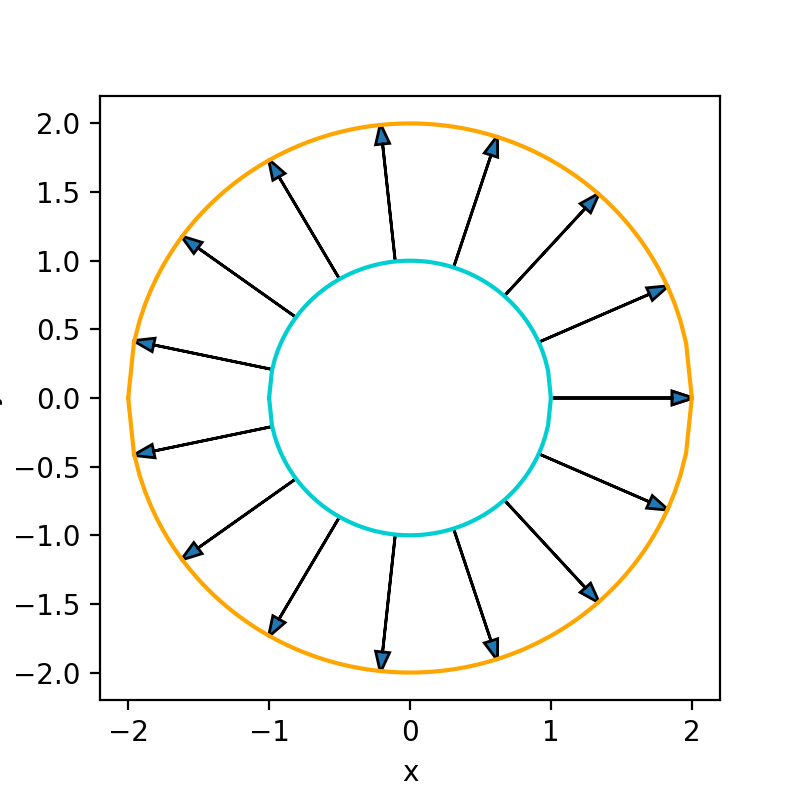
\includegraphics{imagens/ex-8.png}
  \caption{Diagrama das linhas de força no interior das superfícies, secção transversal.
  Os eixos estão em unidades de $R$.}
  \label{fig:ex-8-forca}
\end{figure}
\section{Questão 9}
\label{sec:org88406d9}
Um disco muito fino de raio \(a\) está carregado com densidade superficial
uniforme \(\sigma\). Escolha um sistema de coordenadas com origem no centro do
disco e eixo \(z\) perpendicular ao plano do disco. Calcule o campo
elétrico num ponto \(P\) com coordenadas \((0,0,z)\). Para que valor tende o
campo quando \(z\rightarrow0\)? Fisicamente, você acha que esse resultado faz
sentido?

\begin{figure}[h!]
  \centering
  \begin{tikzpicture}
    \draw[thick,fill=red!50,opacity=0.8] (2,0,0) arc (0:360:2 and 1);
    \draw[->] (0,0,0) -- (0,3,0) node[right] {$z$};
    \filldraw[black] (0,2.5,0) circle (2pt) node[right] {$P$};
  \end{tikzpicture}
  \caption{Diagrama da questão 9.}
  \label{fig:ex-9}
\end{figure}
Vamos considerar diversos anéis infinitesimais de raio \(r\) e espessura
\(dr\), concêntricos. Cada anel terá uma carga \(dq = \sigma2\pi rdr\). O campo que
cada anel realiza sobre o ponto \(P\) é
\begin{align*}
  d\mathbf E &= \frac{dq(-r\hat r+z\hat z)}{4\pi\varepsilon_0(r^2+z^2)^{3/2}}\hat z\\
             &= \frac{\sigma rdr}{2\varepsilon_0(r^2+z^2)^{3/2}}z\hat z. 
\end{align*}
Por argumentos de simetria, só há campo na direção \(\hat z\).
Integrando sobre o raio de \(0\) a \(a\), temos
\begin{align*}
  \mathbf E = \frac{\sigma z\hat z}{2\varepsilon_0}\int_0^a \frac{rdr}{(r^2+z^2)^{3/2}}.
\end{align*}
Com a mudança de variáveis \(u=r^2+z^2\), \(du = 2rdr\), temos a integral
\begin{align*}
  \mathbf E &= \frac{\sigma z\hat z}{2\varepsilon_0}\frac12\int_{z^2}^{a^2+z^2} \frac{du}{u^{3/2}}\\
            &= -\frac{\sigma z\hat z}{2\varepsilon_0}\frac12 2{u^{-1/2}}\big\vert_{z^2}^{a^2+z^2}\\
            &= -\frac{\sigma z\hat z}{2\varepsilon_0}\left(\frac1{\sqrt{a^2+z^2}}-\frac1z\right).
\end{align*}
Com \(z^2 \ll a^2\), a raiz se aproxima de a. Então
\begin{align*}
  \mathbf E &\approx -\frac{\sigma z\hat z}{2\varepsilon_0}\left(\frac1a-\frac1z\right)\\
            &= -\frac{\sigma z\hat z}{2\varepsilon_0}\left(\frac{z-a}{az}\right)\\
            &\approx -\frac{\sigma z\hat z}{2\varepsilon_0}\left(\frac{-1}{z}\right)\\
            &= \frac{\sigma \hat z}{2\varepsilon_0}.
\end{align*}
Quando muito próximo do disco, o campo se aproxima do campo de um plano
carregado. 
\section{Questão 10}
\label{sec:orgc6b5260}
Uma esfera maciça de raio \(R\) tem carga elétrica uniformemente
distribuída em seu interior, de forma que a densidade volumétrica de
carga seja \(\rho\). Em outras palavras, qualquer volume \(\Delta V\) no interior da
esfera tem carga \(\Delta q=\rho\Delta V\). Calcule o campo elétrico num ponto \(P\) da
esfera a uma distância \(r<R\) do centro. \emph{Sugestão. Imagine uma}
\emph{superfície de raio \(r\) cujo centro coincida com o da esfera e aplique}
\emph{nela a Lei de Gauss.}

Utilizando a Lei de Gauss para um sistema similar ao da Figura
\ref{fig:ex-5}, com a esfera interna maciça, temos
\begin{align*}
  \oint \mathbf E\cdot d\mathbf S &= \frac{Q_{in}}{\varepsilon_0}\\ 
  |\mathbf E| 4\pi r^2 &= \frac{4\pi R^3\rho}{3\varepsilon_0}\\
  |\mathbf E| &= \frac{\rho R^3}{3\varepsilon_0r^2}.
\end{align*}
Poderíamos ter calculado o campo para pontos interiores à esfera de raio
\(R\). A única diferença em relação as contas anteriores seria que
\(Q_{in}=4\pi r^3 \rho/3\). Assim,
\begin{align*}
  |\mathbf E| 4\pi r^2 &= \frac{4\pi r^3\rho}{3\varepsilon_0}\\
  |\mathbf E| &= \frac{\rho r}{3\varepsilon_0}.
\end{align*}
Veja que o campo elétrico em tal situação é contínuo. 
\begin{verbatim}
import matplotlib.pyplot as plt
import numpy as np
from matplotlib.pyplot import figure
figure(dpi=250)

def e_dentro(r):
    return r/3

def e_fora(r):
    return 1/(3*r**2)

x_d = np.linspace(0,1,20)
x_f = np.linspace(1,5,35)
plt.plot(x_d,e_dentro(x_d))
plt.plot(x_f,e_fora(x_f))
plt.xlabel(r"$r/R$")
plt.ylabel(r"$|E(r)|$ em unidades de $\rho/\varepsilon_0$.")
plt.legend([r"$r<R$",r"$r>R$"])
plt.savefig("imagens/ex-10.png")
\end{verbatim}
\begin{figure}[h!]
  \centering
  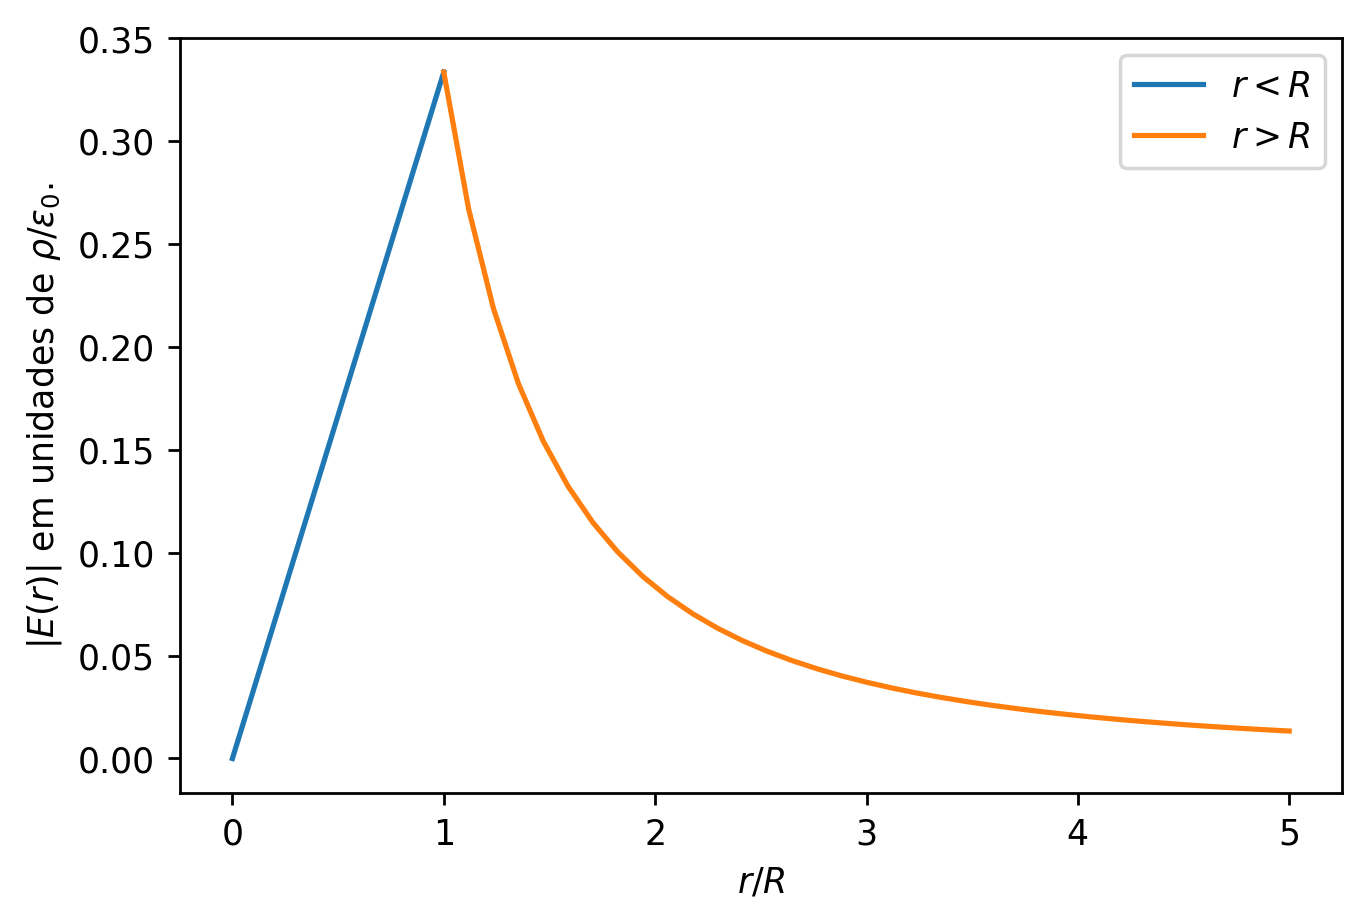
\includegraphics[scale=0.8]{imagens/ex-10.png}
  \caption{Intensidade do campo em função da distância ao centro da esfera.}
\end{figure}
\end{document}